\scanpage{12}
Donnée de $q$ équivaut : la donnée de $\sigma\in\operatorname{Aut}^{\pm1}(\unsure{G|Z},T)$
\[
\left\{\begin{aligned}p(\sigma)&=-1\\ \sigma^2&=1\end{aligned}\right.
\]
\[
\begin{aligned}
&q_t(-1)=\sigma_t\\
&\sigma_{tg}=g\,\sigma_t\,g^{-1}
=g\,\underbrace{\sigma_t\,g^{-1}\,\sigma_t^{-1}}_{g}\,\sigma_t
=g^2\,\sigma_t=\sigma_t\,g^{-2}\\
&\hspace{18em}\boxed{\sigma_{tg}=g^2\sigma_t=\sigma_t g^{-2}}
\end{aligned}
\]

\uline{Corollaire} Si $n$ impair, $t\longmapsto\deleted{\unsure{q}}\sigma_t$ est une bijection de $T$ avec l'ens \deleted{\unsure{des}} $p^{-1}\{-1\}$; donc si on a un \unsure{pl.|pol.} à un nb impair de cotés, l'applic\textsuperscript{n} $t\longmapsto\sigma_t$ qui, à tt sommet du polygone, associe l'unique \unsure{autom|autom.} non orienté qui fixe ce sommet, est bijection.

% slanted left margin note; text rises to the right by approximately 31 degrees.
\reversemarginpar
\margin{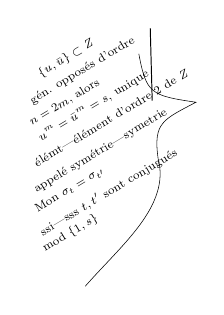
\begin{tikzpicture}[x=.005cm,y=-.005cm,baseline=(mone.base)]
\node[anchor=west,rotate=31,font=\scriptsize,scale=.6,inner sep=0pt] (mone) at (30,125) {$\{u,\bar u\}\subset Z$};
\node[anchor=west,rotate=31,font=\scriptsize,scale=.6,inner sep=0pt] at (10,193) {gén. opposés d'ordre};
\node[anchor=west,rotate=31,font=\scriptsize,scale=.6,inner sep=0pt] at (8,248) {$n=2m$, alors};
\node[anchor=west,rotate=31,font=\scriptsize,scale=.6,inner sep=0pt] at (31,286) {$u^m=\bar u^m=s$, \uline{unique}};
\node[anchor=west,rotate=31,font=\scriptsize,scale=.6,inner sep=0pt] at (20,350) {\uline{\unsure{élémt|élément} d'ordre} 2 de $Z$};
\node[anchor=west,rotate=31,font=\scriptsize,scale=.6,inner sep=0pt] at (20,418) {appelé \unsure{symétrie|symetrie}};
\node[anchor=west,rotate=31,font=\scriptsize,scale=.6,inner sep=0pt] at (23,469) {Mon $\sigma_t=\sigma_{t'}$};
\node[anchor=west,rotate=31,font=\scriptsize,scale=.6,inner sep=0pt] at (35,526) {\unsure{ssi|sss} $t,t'$ sont \unsure{conjugués}};
\node[anchor=west,rotate=31,font=\scriptsize,scale=.6,inner sep=0pt] at (42,568) {mod $\{1,s\}$};
% The short heavy side rule and the thinner extended curve are separate strokes.
\draw[line width=.35pt] (313,6)--(318,190);
\draw[line width=.2pt] (284,71) .. controls (303,172) and (314,177) .. (429,194)
 .. controls (346,238) and (320,245) .. (333,337)
 .. controls (365,457) and (240,556) .. (148,661);
\end{tikzpicture}}
\normalmarginpar
\uline{NB} Si $n$ pair, \unsure{\deleted{elle}|elle} \unsure{ce} n'est pas bijectif, \deleted{mais} \deleted{\unsure{pour tt}} ses fibres sont vides ou de cardinal 2\ldots

\uline{Sommet} \uline{opposé}, symétrie canonique

\uline{Parenthèse}\qquad Produit fibré d'ens

\diagram{\begin{tikzpicture}[x=1cm,y=1cm]
\node (E) at (0,1.2) {$E$};
\node (S) at (1.8,1.2) {$\unsure{S|B}$};
\node (P) at (0,0) {$P$};
\node (F) at (1.8,0) {$F$};
\draw[->] (E)--node[above] {$p$} (S);
\draw[->,dashed] (P)--node[left] {$q'$} (E);
\draw[->,dashed] (P)--node[above] {$p'$} (F);
\draw[->] (F)--node[right] {$q$} (S);
\node[anchor=west,inner sep=0pt] at (4.2,0) {$P\subset E\times F$};
\node[rotate=90,inner sep=0pt] at (4.35,-.55) {$=$};
\node[anchor=west,inner sep=0pt] at (4.05,-1.05) {$\{(x,y)\mid px=qy\}$};
% Detached dark pair at the far right: writing versus surface trace remains open.
\node[inner sep=0pt] at (10.2,-.65) {\unsure{\tikz[x=1pt,y=1pt,baseline=0pt]{\fill (0,0) circle (.4);\fill (2,3) ellipse (.45 and .6);}}};
\end{tikzpicture}}

% Detached hooked pen stroke above Solution; no letter or mathematical role assigned.
\figure{\begin{tikzpicture}[x=1cm,y=1cm]
\path[use as bounding box] (0,0) rectangle (13,.4);
\fill (.105,.29) ellipse (.025 and .045);
\draw[line width=.7pt,line cap=round] (.10,.30) .. controls (.09,.22) and (.16,.18) .. (.13,.13) .. controls (.11,.08) and (.08,.09) .. (.07,.10);
\end{tikzpicture}}

Solution d'un Pb universel dans la cat. des ens :

Si $E,F,S$ des \unsure{grpes|groupes}, $p,q$ hom de \unsure{grpe|groupe}, alors $P$ un \unsure{grpe|groupe} (et solution du pb univ. analogue \unsure{ds|dans} cat. des \unsure{grpes|groupes})
\[
\operatorname{Ker}p\sim\operatorname{Ker}p',\quad
\operatorname{Ker}q\sim\operatorname{Ker}q'
\]

% The raised addition and the curved stroke below it sit over the start of surjectif.
% The first closing parenthesis is written without a distinct opening one.
Si \tikz[baseline=(base.base)]{
\node[anchor=base west,inner sep=0pt] (base) at (0,0) {$p$ surjectif};
\node[anchor=base west,inner sep=0pt] at (.27,.46) {\inserted{$:E\mathbin{\text{---}}S$}};
\draw[line width=.25pt] (.44,.12) .. controls (.70,.34) and (1.08,.28) .. (1.58,.41);
} bijectif) alors $P\mathbin{\text{---}}F$ surjectif (bijectif).

[Langage des \tikz[baseline=(old.base)]{
\node[anchor=base,inner sep=0pt] (old) at (0,0) {\deleted{\unsure{diagrammes}}};
\node[anchor=base,inner sep=0pt] at (0,.40) {\inserted{carrés}};
} cartésiens]

Image inverse d'ex. de \unsure{grpe|groupe|grpes|groupes}
% archive sheet number: 11
